
\documentclass[11pt,a4paper]{article}
\usepackage[left=2cm,right=2cm,top=2cm,bottom=3cm]{geometry}
\usepackage{amsmath,amsfonts,amsthm,amssymb,varioref,times, commath}
\usepackage{gensymb}
\usepackage{tikz}
\usepackage{textcomp}
\usepackage{hyperref}
\hypersetup{
 colorlinks=true,
 linkcolor=blue,
 filecolor=magenta, 
urlcolor=cyan,
}
\usepackage{lipsum}
\usepackage{epigraph}
%to resume numbering in a list
\usepackage{enumitem}
%----- arrows 
\usepackage{extarrows}

%    differential equatiosn 
\usepackage{diffcoeff}   %\diff[2]{x}{y}


%%%%%%pour ecrire en français avec les accents
\usepackage[utf8]{inputenc}
\usepackage[T1]{fontenc}
\usepackage{lmodern} % load a font with all the characters
\usepackage{units}
%%%%%%%Image-related packages
\usepackage{wrapfig}
\usepackage{float, graphicx}
\graphicspath{ {./img/} }
\usepackage{subcaption}
\usepackage[export]{adjustbox}

%%%%%%%pour faire des cadres
\usepackage{xcolor}
\usepackage{tcolorbox}
\usepackage{framed}
\usepackage{mdframed}


%%%%%%%chemistry frmulae
\usepackage{chemfig}
\usepackage{chemformula}
\usepackage[version=4]{mhchem}

% -------------- Circuits -------------------
\usepackage[european, straightvoltages]{circuitikz}

% Title & headers
\usepackage[explicit]{titlesec}
% Raised Rule Command:
% Arg 1 (Optional) - How high to raise the rule
% Arg 2 - Thickness of the rule
\newcommand{\raisedrulefill}[2][0ex]{\leaders\hbox{\rule[#1]{1pt}{#2}}\hfill}
\titleformat{\section}{\Large\bfseries}{\thesection. }{0em}{#1\,\raisedrulefill[0.4ex]{1pt}}

% pour ecrire sur +sieurs colonnes
\usepackage{multicol}
\setlength{\columnseprule}{0pt}
\setlength{\columnsep}{60pt}
% Fusion de lignes de tableaux.
\usepackage{multirow}
% Position verticale des lettres dans la ligne de tableau.
\usepackage{array}

% physics -----------------------------------------------------------
\newcommand{\To}{\longrightarrow}
\newcommand{\gpl}{\; g\cdot L^{-1}}
\newcommand{\gpmol}{\; g\cdot mol^{-1}}
\newcommand{\mpl}{\; mol\cdot L^{-1}}
\newcommand{\mps}{\; m\cdot s^{-1}}
\newcommand{\rps}{\; rad\cdot s^{-1}}
\newcommand{\kph}{\; km\cdot h^{-1}}
\newcommand{\mpss}{\; m\cdot s^{-2}}
\newcommand{\Dt}{\Delta t}
\newcommand{\vv}{\vec{v}}
\newcommand{\va}{\vec{a}}
\newcommand{\vp}{\vec{p}}
\newcommand{\vf}{\vec{F}}
\newcommand*{\Vf}[1]{\overrightarrow{F_\ensuremath{{#1}}}}
\newcommand{\es}[1]{\cdot10^{#1}}
\newcommand{\eng}[1]{\textcolor{purple}{(= #1})}
\usepackage{harpoon}
%\newcommand*{\vect}[1]{\overrightharp{\ensuremath{#1}}}
\newcommand*{\Vect}[1]{\overrightarrow{\ensuremath{#1}}}
\newcommand{\pfd}[1]{\sum \vec{F}_{ext_{#1}} &= \od{\vp_{#1}}{t} = m\cdot\va_{#1}}
\newcommand{\C}{\degree C}
\newcommand{\Delt}{\Delta t}

% --- Circuits ------------
\newcommand{\bipole}[1]{
\begin{circuitikz} \draw
(0,0) to[ #1 ] (2,0); 
\end{circuitikz} {\hspace{5mm}}}

% Chimie ---------------------------------
\newcommand{\oxo}{\ce{H3O+}_{(aq)}}
\newcommand{\eau}{\ce{H2O}_{(\ell)}}
\newcommand{\OH}{\ce{HO-}_{(aq)}}
\newcommand{\AH}{\ce{AH}_{(aq)}}
\newcommand{\A}{\ce{A-}_{(aq)}}
\newcommand{\MnO}{\ce{MnO_4^{-}}}
\newcommand{\conc}[1]{\left[{#1}\right]}
\newcommand{\couple}[2]{\ce{#1/#2}}


% Environnements ------------------------
\newcounter{exo}
\newenvironment{exo}[1][]
{\refstepcounter{exo} \begin{shaded}\noindent $\triangleright \quad$\textbf{Exercice~\theexo. #1} } { \end{shaded}}
\newenvironment{eg}
{\begin{shaded} \textbf{Exemple:} } { \end{shaded}}

\newenvironment{defn}[1]
{\begin{leftbar}\noindent \textbf{Définition :\textit{ \quad #1}} } { \end{leftbar}}

%\newenvironment{rmrq}
%{\begin{shaded} \textbf{Remarque.\quad } \itshape } { \end{shaded}}
\newenvironment{rmrq}
{\begin{mdframed}[backgroundcolor=blue!10, linewidth=0pt] \textbf{Remarque.\quad } \itshape } { \end{mdframed}}

\newenvironment{python}
{\begin{shaded} \textbf{A faire en PYTHON}\\ \itshape } { \end{shaded}}

% Shading colour -----------------------------
\definecolor{shadecolor}{gray}{0.9}

\date{}
\author{}

\renewcommand*\contentsname{Résumé}









% Title & headers 
\usepackage{fancyhdr}
\pagestyle{fancy}
\fancyhf{}
\lhead{SciPhy : Terminale spé}
\rhead{Ch. 4 : Cinétique chimique}
\chead{2020-28}
\rfoot{Page \thepage}
\lfoot{\textcopyright\; S Zayyani}
\renewcommand{\footrulewidth}{0.1pt}% default is 0pt

\title{\large Chimie - Chapitre 4 \\ \LARGE La cinétique chimique \\ \small Vitesses des réactions}
\date{}
\author{}

\setlength{\parindent}{0mm}
\setlength{\parskip}{2mm}

%%%%%%%%%%% For wrapfigure 
\setlength{\intextsep}{6pt}%
\setlength{\columnsep}{3pt}%



\begin{document}
\maketitle
\vspace{-2cm}
\begin{tcolorbox}[title=Notions de la classe de première à rappeler]
calcul d'un logarithme ; solvatation d'un proton libre dans l'eau ; Concentration molaire ; dérivée d'une fonction ; équation différentielle de premier degré 
%\tcblower
\end{tcolorbox}
\vspace{1cm}
\tableofcontents
\vspace{1cm}
\section{Étude qualitative}

Nous entamons ici un nouveau domaine de la chimie, l'étude de la vitesse et de la dynamique des réactions. Jusqu'alors nous avons supposé que toute réaction étaient instantanée. Nous savons que ceci n'est pas le cas, car nous connaissons des réactions vives (comme la combustion) mais aussi des réaction qui peuvent avoir lieu pendant une période très longue (comme la corrosion). Commençons donc par quelques définitions. 

\subsection{Réactions lentes \& rapides}
\begin{defn}{Réaction rapide \& lente}
\begin{itemize}
    \item La durée d’une réaction est le temps nécessaire pour l’évolution du système entre deux états. 
    \item Si la durée d’évolution d’un système est trop courte pour pouvoir être mesurée, la transformation est dite rapide (par rapport à la technique de mesure)
    \item Si une technique permet de mesurer la durée d’évolution d’un système, la transformation est dite lente (par rapport à la technique de mesure). 
    \item Généralement on considère qu’une transformation qui dure moins d’une seconde est rapide. 
    \item La cinétique chimique est l’étude de l’évolution temporelle des transformations chimiques. 
\end{itemize}
\end{defn}
\begin{eg}

Une \textbf{combustion} est une réaction rapide (considérée même comme instantanée), tandis que la \textbf{formation de la rouille} (qui est une réaction aussi avec le dixoygène) est une réaction lente. 
\end{eg}

\subsection{Facteurs cinétiques}

\begin{defn}{Facteurs cinétiques}
\begin{itemize}
    \item Un facteur cinétique est un \textbf{paramètre qui influence} la vitesse d’une réaction, et donc la durée d’une réaction.
    \item Un facteur cinétique pourrait être un paramètre \textbf{physique} ou \textbf{chimique}.
\end{itemize}
\end{defn}
	
Les facteurs cinétiques principaux sont :
\begin{itemize}
        \item \textbf{La température du système : }l’évolution d’un système chimique est d’autant plus rapide que sa température est élevée. Ceci est du au fait que, aux températures plus élevées, le nombre de chocs, et surtout l'énergie des chocs entre les molécules augmente.
        \item \textbf{La concentration des réactifs : }l’évolution d’un système chimique est d’autant plus rapide que les concentrations des réactifs sont élevées. En effet, quand le nombre d’entités chimiques contenues dans un volume donné augmente, la fréquence des chocs augmente et la probabilité d’un choc efficace également.  (A-ha ! Et cela explique aussi pourquoi la vitesse de la réaction diminue au cours de la réaction !)
        \item \textbf{L’état physique de la matière :} l’état physique influence aussi le contact entre les molécules. Les réactifs ont plus de surface de contact à l’état liquide, par exemple, qu’à l’état solide, et donc plus de possibilité de chocs efficaces.
        \item \textbf{La présence d’un catalyseur }
        \item \textbf{Le choix du solvant : }Le solvant (comme le catalyseur) n’apparait pas dans le bilans des matières d’une réaction chimique, et pourtant son influence sur la vitesse d’une réaction pourrait être très importante. Un solvant qui solubilise bien des espèces chimiques, favorise leur contact, et rend donc la réaction plus rapide. 
        \item \textbf{La nature des entités }(i.e. la structure géométrique et la forme des molécules) 
        \item Divers facteurs (L’éclairement du milieu réactionnel, agitation, …)
    \end{itemize}

\subsection{Catalyse}

\begin{defn}{Catalyse\eng{Catalysis}}
\begin{itemize}
    \item La \textbf{catalyse} est le phénomène de modification de la vitesse d'une réaction chimique par l'action d'une substance appelée \textbf{catalyseur}
    \item La catalyse peut aussi avoir un effet sur la sélectivité d'une réaction chimique dans le cas de réactions concurrentes en favorisant la production d'un produit plutôt qu'un autre. 
    \item Un \textbf{catalyseur} \eng{catalyst} est une espèce chimique qui augment la vitesse d’une réaction chimique (i.e. diminue la durée d’une réaction), mais qui \textbf{ne figure pas dans l’équation de cette réaction.}
    \item Le catalyseur, est en général en quantité beaucoup plus faible que les réactifs. 
    \item Explication : Un catalyseur « fragilise » certaines liaisons, et par conséquent leur rupture a besoin de beaucoup moins d’énergie, et du coup a lieu plus facilement et plus rapidement.
\end{itemize}
\end{defn}

Il existe plusieurs formes de catalyse, mais on parle généralement de trois types : 

\begin{itemize}
    \item \textbf{Catalyse hétérogène : } Lorsque le réactif et le catalyseur sont dans des états physiques différents. 
    
    En catalyse hétérogène, la surface de contact entre le catalyseur et les réactifs, appelée \textbf{surface active}, joue un rôle essentiel, car c’est à cette surface-là que les entités chimiques interagissent. 
    
    En catalyse hétérogène, un catalyseur est d’\textbf{autant plus efficace que sa surface active est grande. }
    
    Exemple : La réaction de synthèse de l'eau à partir du dihydrogène et du dioxygène peut être catalysée par le platine solide (mousse de platine). Les réactifs sont en phase gazeuse et le catalyseur est en phase solide. $\ce{2 H2 + O2 ->[Pt] 2 H2O }$
    
    \item \textbf{Catalyse homogène : } Lorsque le catalyseur et les réactifs sont tous gazeux ou tous en solution aqueuse, il s’agit de catalyse homogène. 
    
    En catalyse homogène, un catalyseur est d’autant plus actif que sa concentration est grande. 
    
    Exemple :  La réaction de décomposition (dismutation) de l'eau oxygénée peut être catalysée par les ions fer (III) en solution aqueuse. Il n’y a qu'une seule phase, la phase aqueuse : $\ce{2 H2O2 ->[Fe^{3+}_{(aq)}] 2 H2O + O2}$
    \item \textbf{Catalyse enzymatique : }Lorsque qu’une réaction est catalysée par une enzyme, il s’agit d’une catalyse enzymatique.
    
    Dans une catalyse enzymatique les réactifs sont en solution dans le même milieu que le catalyseur. La catalyse enzymatique est donc un cas particulier de catalyse homogène. 
    
    Les enzymes sont des catalyseurs très sélectifs, et très efficaces. 
\end{itemize}
	
\section{Étude quantitative}

Jusqu'alors nous avons parlé de manière très qualitative des notions autour de la vitesse d'une réaction. Passons donc à une approche plus quantitative et analytique, qui nous permettra de développer des outils pour caractériser mathématiquement la cinétique des réactions chimiques. 

\subsection{Suivi temporel d'une réaction chimique}

Le suivi temporel d’une transformation permet d’obtenir l’évolution au cours du temps de la concentration molaire ou de la quantité de matière d’un réactif ou d’un produit.  Si l’on connaît l’équation de la réaction, il est possible d’obtenir l’évolution temporelle de l’avancement chimique. Pour la réaction suivante, par exemple :

\begin{figure}[h]
    \centering
    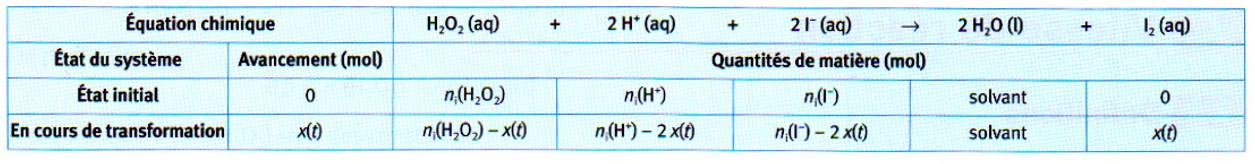
\includegraphics[width=\linewidth]{imgs/c4/tableau.jpg}
\end{figure}
\begingroup
\begin{wrapfigure}{r}{0.5\textwidth}
  \centering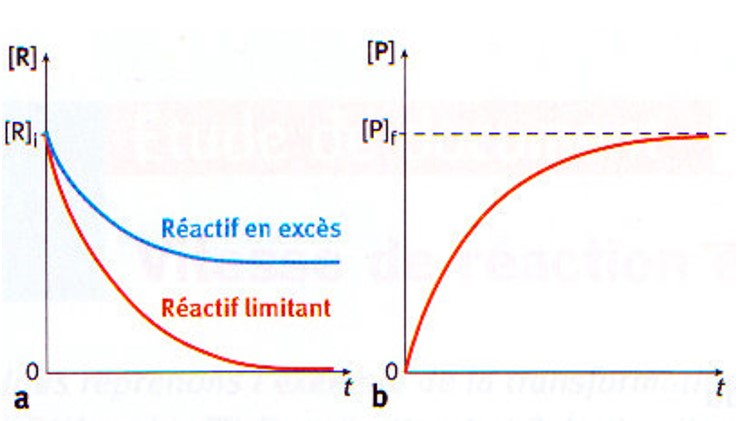
\includegraphics[width=0.95\linewidth]{imgs/c4/reactlimit.jpg}
\end{wrapfigure}

Et on a donc les expressions de la quantité de matière en fonction du temps suivantes : 
\begin{align*}
    n({\ce{H2O2}})\left(t\right) &= n_i({\ce{H2O2}})\left(t\right) - x(t) \\
    n({\ce{H+}})\left(t\right) &= n_i({\ce{H+}})\left(t\right) - 2x(t) \\
    n({\ce{I-}})\left(t\right) &= n_i({\ce{I-}})\left(t\right) - 2x(t) \\
    n({\ce{I2}})\left(t\right) &= x(t) \\
\end{align*}
Nous pouvons visualiser ces évolutions, graphiquement, de la manière suivante :

\endgroup
Évidemment les quantités de matière des réactifs diminuent, d’où les courbes décroissantes ; et les quantités de matière des produits augmentent, d’où les courbes croissantes. 

Constatons qu’en général la vitesse de réaction diminue au cours d’une transformation et tend vers zéro quand $t$ tend vers l’infini.  Ceci est dû aux facteurs cinétiques, que nous avons vu précédemment. 

Les méthodes expérimentales de suivi sont les mêmes que nous avons déjà vue : la conductimètrie, la spectrophotométrie, des titrages.  Dans tous les cas, la méthode permet un suivi de l'évolution de la concentration, que l'on peut suivre avec un repérage temporel. 


\subsection{Temps de demi-réaction}

\begin{defn}{Temps de demi-réaction}
\begin{itemize}
    \item Le temps de demi-réaction, noté $t_(1⁄2)$, correspond à la durée nécessaire pour que l’avancement de la réaction atteigne la moitié de sa valeur finale, soit :
    \[ x\left( t_{1/2} \right) = \frac{x_{final}}{2}       \]
    \item Dans le cas d’une réaction totale, la valeur finale de l’avancement est égale à l’avancement maximal, c’est-à-dire : 
    \[ x\left( t_{1/2} \right) = \frac{x_{final}}{2} = \frac{x_{max}}{2}      \]
    Ce temps correspond alors au temps nécessaire pour consommer la moitié de la quantité initiale de réactif limitant. 
	\item \textbf{ATTENTION : }Le temps de demi-réaction N’EST PAS égal à la moitié de la durée de réaction. 
\end{itemize}
\end{defn}

Nous allons voir par la suite une méthode analytique pour déterminer le temps de demi-réaction, mais il y a un moyen très facile de faire la lecture de la valeur, si nous disposons d'un graphique de l'évolution de la concentration (ou de la quantité de matière) en fonction du temps. Il suffit de lire par projection de la courbe, la date correspondant la valeur de concentration $\frac{[x]_{final}}{2} $. 
\begin{figure}[h]
    \centering
    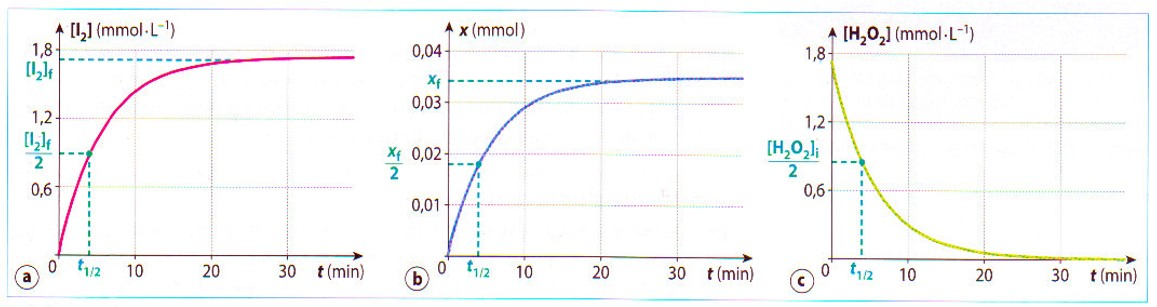
\includegraphics[width=\linewidth]{imgs/c4/demitemps.jpg}
\end{figure}

\begin{figure}[h]
    \centering
    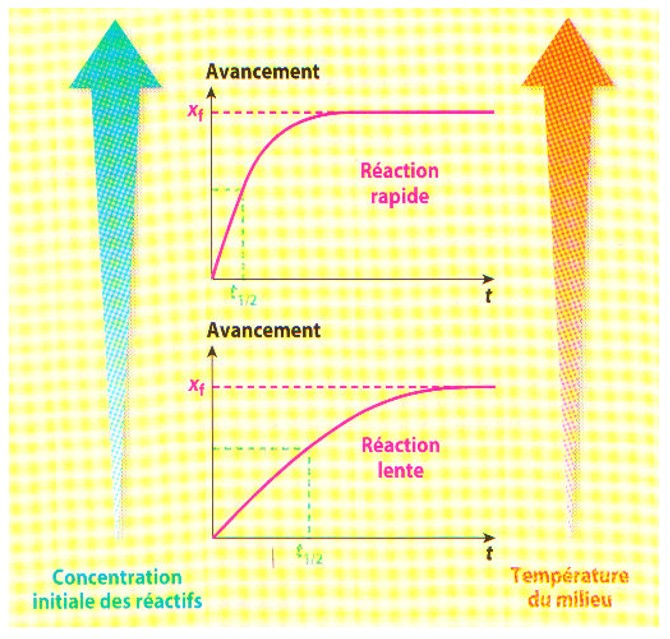
\includegraphics[width=0.7\linewidth]{imgs/c4/vitelente.jpg}
    \caption{Pour une même avancement final, deux réactions n'ont pas la même vitesse d'avancement. }
\end{figure}

\begin{rmrq}
En règle générale, pour une réaction chimique qui suit une courbe exponentielle, on peut dire qu'une réaction atteint son état final au bout d'une durée de $5\;t_{1/2} $.
\end{rmrq}
\subsection{Vitesse volumique}

Nous allons commencer par définir une grandeur importante qui va nous permettre de mesure de taux de variation d'une espèce chimique. Ce qui va suivre - pas étonnement - va ressembler beaucoup à ce que nous avons fait en \textit{cinématique}; ce qui est logique car nous utiliserons le même langage : les taux de variation d'une grandeur (la position en cinématique, les quantités de matière ou des concentrations en cinétique chimique). 

\begin{defn}{Vitesse d'apparition/disparition d'une espèce chimique}
\begin{itemize}
    \item La vitesse d'apparition ou de formation d'un produit $P$, est donnée par : 
    \[ v_{formation}(\ce{P}) = \od{\left[\ce{P}\right]}{t}       \]
    \item La vitesse de disparition d'un réactif $R$, est donnée par : 
    \[ v_{disparition}(\ce{R}) = - \od{\left[\ce{R}\right]}{t}       \]
\end{itemize}
\end{defn}

\begin{defn}{Vitesse volumique moyenne/instantanée}
\begin{itemize}
    \item la vitesse volumique est la différences entre les quantités de matière dans un mélange réactionnel, entre deux instants. 
    \item la vitesse moyenne volumique $v$ du produit $\ce{X}$ entre les dates $t_1$ et $t_2$ est donnée par : 
    \[ v_x(t) = \frac{1}{V}\od{x}{t} \quad \text{où}\quad \begin{cases}
    x \rightarrow \text{avancement de réaction en }(\mpl) \\
    V \rightarrow \text{Volume du milieu en }(L) \\ 
     \end{cases} \]
    \item la vitesse volumique s'exprime en $\mpl\cdot s^{-1}$ 
\end{itemize}
\end{defn}

La vitesse volumique peut être déterminé graphiquement, car, comme vous savez déjà, la dérivée d'une fonction représente le coefficient directeur de la tangente à la courbe représentée par la fonction, à l'instant considéré (c.f. figures suivantes). 

\begin{figure}[ht]
\centering
\begin{subfigure}{.45\textwidth}
  \centering
  % include first image
  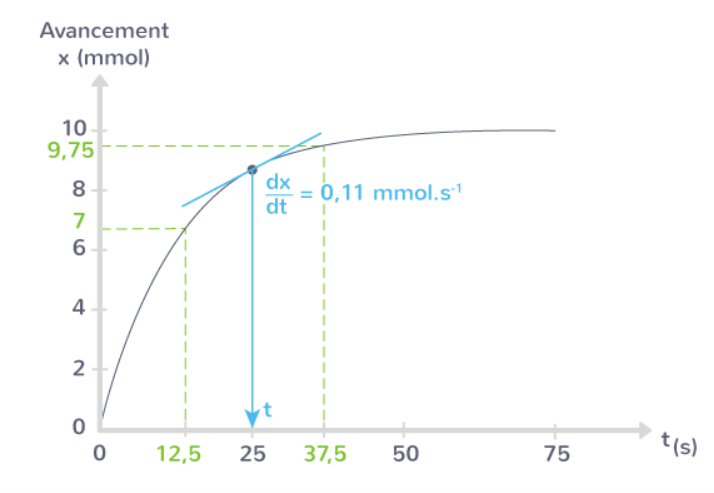
\includegraphics[width=.95\linewidth]{imgs/c4/tangente1.png}  
\end{subfigure}
\begin{subfigure}{.45\textwidth}
  \centering
 %%%%%%%%%%% % include first image
  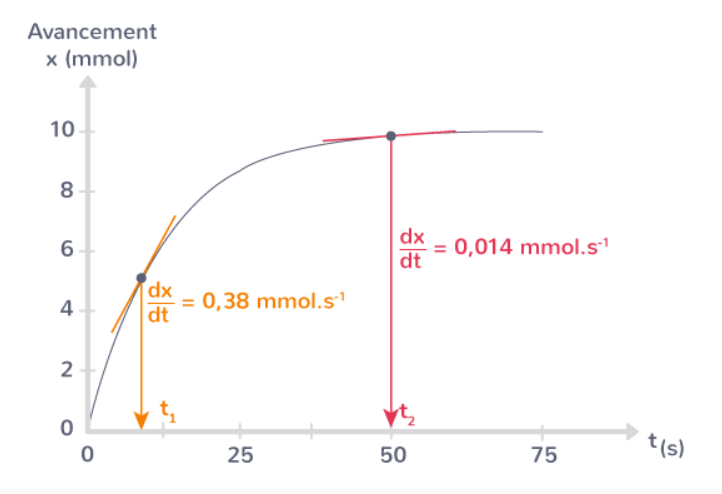
\includegraphics[width=.95\linewidth]{imgs/c4/tangente2.png}  
\end{subfigure}
\caption{Variation de $i$ et de $r$ pour un rayon passant de l'air dans le verre.}
\end{figure}

\begin{rmrq}
A moins que le courbe de l'évolution de l'avancement de réaction de réactions soit une droite (i.e. constante, ce qui n'est presque jamais de cas), nous voyons sur les figures précédente que la vitesse de réaction change constamment; et que la plupart du temps, elle diminu au cours de la réaction.   
\end{rmrq}

Considérons maintenant la réaction suivante :  $ \ce{H2O2_{(aq)}} + \ce{2H+ + 2I^-_{(aq)} -> 2H2O_{(\ell)} + I2_{(aq)}} $

L'avancement de la réaction peut s'exprimer : $x(t) = n_i\left(\ce{H2O2}\right) - n\left(\ce{H2O2}(t)\right)$

d'où l'expression de la vitesse de la réaction: 
\[ v(t) = -\frac{1}{V}\od{\;n(\ce{H2O2})}{t} =-\od{\conc{\ce{H2O2}}}{t}
\]

Mais ce même avancement peut s'exprimer aussi en termes d'autres espèces, comme l'ion d'hydrogène : $x(t) = \dfrac{n_i\left(\ce{H+}\right) - n\left(\ce{H+}(t)\right)}{2}$ 
\[ v(t) = -\frac{1}{2V}\od{\;n(\ce{H+})}{t} =-\dfrac{1}{2}\od{\conc{\ce{H+}}}{t}
\]
ou encore en terme de l'iode :  $x(t) = \dfrac{n_i\left(\ce{I-}\right) - n\left(\ce{I-}(t)\right)}{2}$ 
\[ v(t) = -\frac{1}{2V}\od{\;n(\ce{I-})}{t} =-\dfrac{1}{2}\od{\conc{\ce{I-}}}{t}
\]

et donc en règle générale, pour une réaction chimique du type $ \ce{aA + bB -> cC + dD}  $ les vitesse de réactions s'expriment : 
\[ v(t) = -\dfrac{1}{a}\od{\conc{A}}{t} = -\dfrac{1}{b}\od{\conc{B}}{t}    \] et 
\[ v(t) = \dfrac{1}{c}\od{\conc{C}}{t} = \dfrac{1}{d}\od{\conc{D}}{t}    \] 

ou encore plus généralement : $v(t) = -\dfrac{1}{a}v_A = -\dfrac{1}{b}v_B = \dfrac{1}{c}v_C = \dfrac{1}{d}v_D $

\subsection{Lois de vitesse d'ordre 1}

\begin{defn}{Loi de vitesse d'ordre 1}
\begin{itemize}
    \item Une loi de vitesse est une équation établissant un lien entre la vitesse volumique d'une réaction et les concentration des réactifs. 
    \item Une loi est \emph{d'ordre 1}, si la vitesse ne dépend que de la concentration d'un seul réactif, et que cette vitesse est proportionnelle à cette concentration. 
    
    C'est à dire une réaction du type : $a\ce{A -> }  b\ce{B} + c\ce{C}$
    \item La loi de vitesse d'ordre 1 par rapport au réactif $\ce{A}$ s'écrit : 
    \[v = k\cdot\conc{A} \]
    \item $k$ s'appelle la \textbf{constante de vitesse}, s'exprime en $s^{-1}$, et est une caractéristique thermodynamique de la réaction. 
\end{itemize}
\end{defn}

Une loi d'ordre 1 est le cas de la plupart des réactions avec un seul réactif, mais peut aussi décrire certaines réaction à deux réactifs. 

Pourquoi parle-t-on alors d'ordre 1? Car cette équation est en fait une \textbf{équation différentielle d'ordre 1}. Rappelons-nous que la vitesse de la réaction est donnée par $ v(t) = \od{\conc{\ce{A}}}{t}$. 

Nous avons donc : 
\begin{align*}
   v &= k\cdot\conc{A} \\
   -\od{\conc{\ce{A}}}{t} &= k\cdot\conc{A} \\
   \od{\conc{\ce{A}}}{t} + k\cdot\conc{A} = 0
\end{align*}

Cette équation est bien une équation différentielle de premier degré. Voilà comment on peut résoudre cette équation: 
\begin{align*}
   -\od{\conc{\ce{A}}}{t} &= k\cdot\conc{A} \\
   \dfrac{d\conc{\ce{A}}}{\conc{\ce{A}}} &= -k\cdot dt 
\end{align*}

\begingroup
\begin{wrapfigure}{r}{0.4\textwidth}
  \centering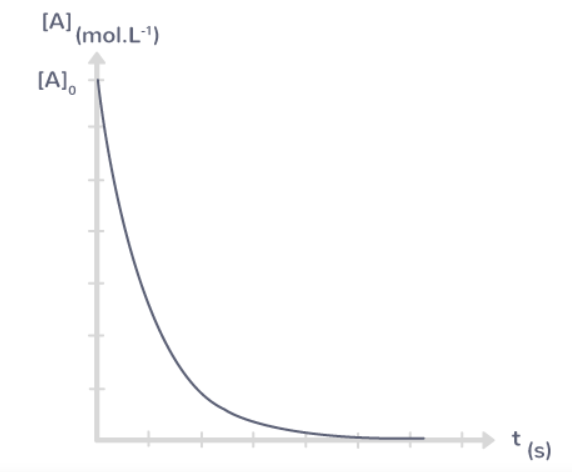
\includegraphics[width=.9\linewidth]{imgs/c4/decroit.png}
\end{wrapfigure}

En intégrant les deux cotés de l'équation avec les conditions initiales $\conc{A}(t=0) = C_0$ on obtient la solution : 
\begin{align*}
    \ln{\dfrac{\conc{A}}{C_0}} &= -k\cdot t \\
    \conc{A} &= C_0e^{-kt}
\end{align*}

Cela correspond bien à une courbe de décroissance exponentielle, que l'on observe expérimentalement souvent, lors d'étude d'une réaction (cf. figure ci-contre).

\endgroup

\begin{eg}
Nous pouvons désormais déterminer l'expression du temps de demi-réaction pour une réaction d'ordre 1. Montrer que pour une telle réaction $t_{1/2} =\frac{0,693}{k}$.
\vspace{3cm}
\end{eg}

\begin{figure}[ht]
\centering
\begin{subfigure}{.48\textwidth}
  \centering
%%%%%%%%%%%%%%%  % include second image
  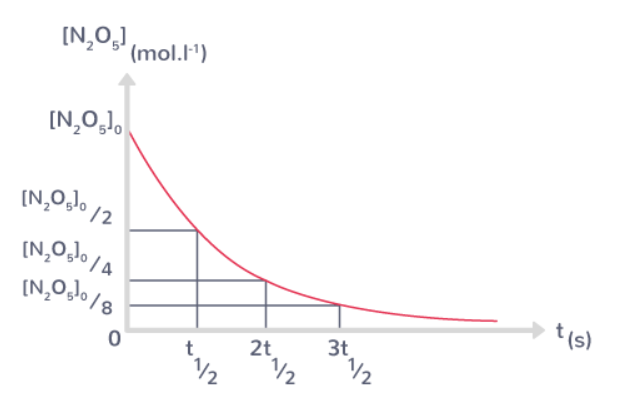
\includegraphics[width=.95\linewidth]{imgs/c4/5demitemps.png}  
\end{subfigure}
\begin{subfigure}{.48\textwidth}
  \centering
  %%%%%%%%%%%%%% include second image
  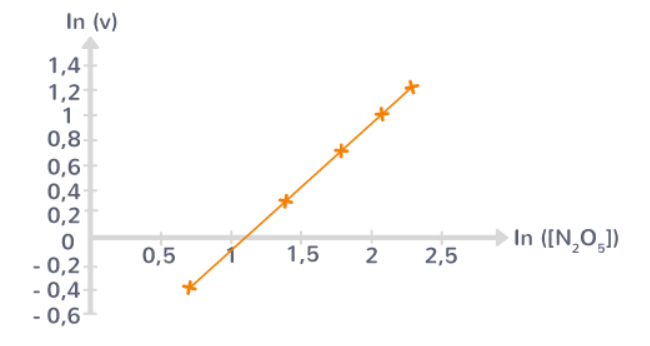
\includegraphics[width=.95\linewidth]{imgs/c4/croitlogarithm.png}  
\end{subfigure}
\caption{Courbe caractéristique d'une décroissance exponentielle. }
\end{figure}

% \subsection{ANNEXE : Lois de vitesse d'ordre $\neq 1$ }

\section{Modélisation microscopique}
Jusqu'alors nous avons essayé de construire un modèle plus ou moins empirique de la cinétique chimique, c'est à dire, nous avons établi un modèle mathématique dont les résultats correspondent à ce que l'on observer et ce que l'on mesure. Ceci est un modèle \emph{macroscopique}. Nous voudrons maintenant construire un modèle \emph{microscopique} de la cinétique chimique, c'est à dire décrire ce qui se passe à l'échelle atomique pour expliquer les observations de la cinétique chimique. 

\subsection{Chocs efficaces}

\begin{quote}
La Théorie des collisions est une théorie qui explique qualitativement comment se produisent les réactions chimiques élémentaires en phase gazeuse et qui rend compte de la dépendance de leur vitesse avec la concentration1. Elle suppose que pour qu'une réaction se produise, les \textbf{molécules des réactifs doivent entrer en collision. Seulement une fraction des collisions se traduisent par la transformation effective des réactifs en produits (on les appelle collisions efficaces). Cela est dû au fait que seulement une partie des molécules ont une énergie suffisante et la bonne orientation au moment de l'impact pour rompre les liaisons existantes et en former de nouvelles} ... La théorie des collisions est ainsi très intimement liée à la théorie cinétique des gaz et constitue un des fondements théoriques de la cinétique chimique.    (Wikipédia)
\end{quote}

\begin{figure}[h]
    \centering
    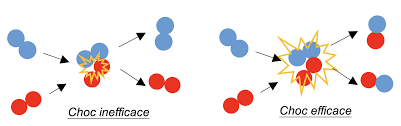
\includegraphics{imgs/c4/chocs.png}
\end{figure}
Pour résumer pour qu'il y ait une réaction chimique entre deux molécules, plusieurs conditions doivent être satisfaites : 
\begin{itemize}
    \item Les deux particules doivent rentrer en contact
    \item Il faut qu'ils possèdent assez d'énergie (énergie d'activation $E_a$) afin de pouvoir briser les liaisons. 
    \item Il faut que les particules soient 'orientées` correctement. 
\end{itemize}

Cette théorie permet donc de faire un lien entre les facteurs cinétiques que nous avons déjà abordés précédemment, et une explication à l'échelle microscopique. 
Par exemple : 
\begin{itemize}
    \item \textbf{Température} : Rappelons-nous que la température est une grandeur - émergent - macroscopique, c'est à dire que les atomes et les molécules n'ont pas de température. La température est, en effet, une mesure de l'énergie cinétique moyenne des particules. Plus la température du milieu s'élève, plus il y a de particules ayant une énergie supérieure au minimum pour que la réaction puisse avoir lieu. 
    \begin{center}
        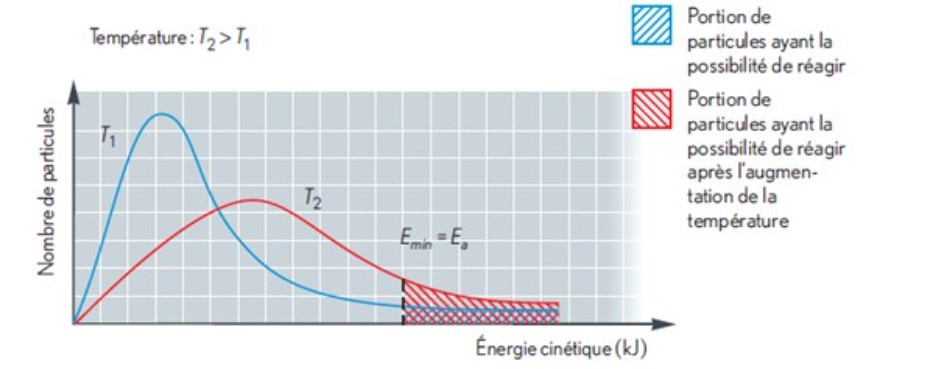
\includegraphics[width=\linewidth]{imgs/c4/energieactivate.jpg}
    \end{center}    
    \item \textbf{Concentration} : Avec une concentration plus élevées, le nombre total de particule avec une énergie nécessaire pour la réaction, est plus élevé, et donc la réaction avance plus rapidement. 
    \item \textbf{Catalyseur} : La présence d'un catalyseur a pour effet une baisse de l'énergie minimum nécessaire pour qu'une collision puisse produire une réaction chimique, et donc pour une température de milieu donnée, un plus grand nombre de particules a suffisamment d'énergie pour la réaction, et donc la vitesse de réaction augmente. 
    \begin{center}
        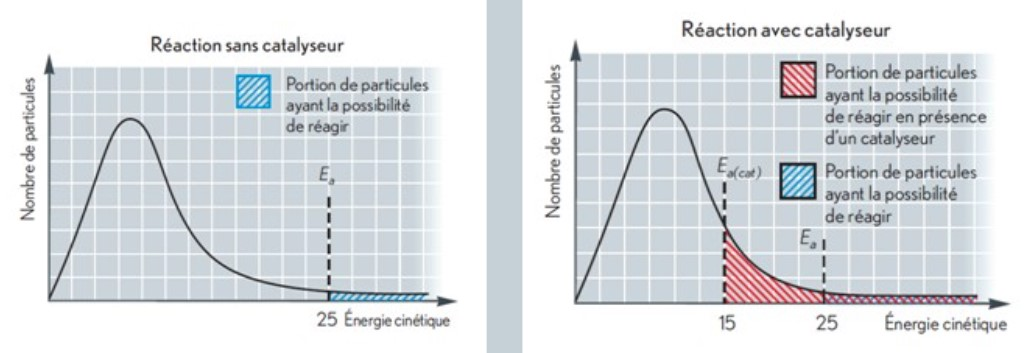
\includegraphics[width=0.9\linewidth]{imgs/c4/energiecatalyse.jpg}
    \end{center}
    \item \textbf{L'état physique des réactifs}. L'état physique des réactifs influence la surface de contact entre eux. A l'état solide seule la surface du solide peut réagir, tandis que à l'état liquide ou gazeux, la surface de contacte augmente, et par conséquences, la vitesse de réaction augmente. 
    \begin{center}
        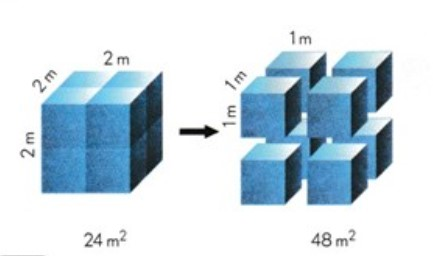
\includegraphics[width=0.6\linewidth]{imgs/c4/surfacecontacte.jpg}
    \end{center}
\end{itemize}

\subsection{Mécanisme réactionnels}

Rappelons-nous qu'une différence importante ($>0,4$)  d'électronégativité entre les atomes dans une liaison covalente, engendre une polarisation de la liaison, et par conséquent une polarisation de la molécule, ou de certaines de ses régions. Ceci, ainsi que la présence ou absence des doublets non-liants, ou encore des liaisons doubles ou triples, créé des régions dans une molécules possédant une \textbf{charge partielle négative $\delta^-$, ou positive $\delta^+$}. 

\begin{defn}{Sites donneurs \& sites accepteurs}

Dans un atome, 
\begin{itemize}
    \item Un \textbf{site donneur} est une zone \textbf{riche en électrons}, et donc \textbf{riche en charge négative}. Ceci peut être en raison d'un excès d'électrons, ou dû à la présence d'un doublet non-liant, ou encore dû à la présence d'une liaison double ou tripe. 
    \item Un \textbf{site accepteur} est une zone \textbf{pauvre en électrons}, et donc \textbf{riche en charge positive}. Ceci peut être en raison d'une absence d'électron, ou d'une polarisation d'une liaison. 
    \item Lors d'une réaction chimique, il y a un \textbf{mouvement d'électrons}. On dit que le \textbf{site donneur attaque le site accepteur}. 
\end{itemize}
\end{defn}
\begin{figure}[ht]
\centering
\begin{subfigure}{.45\textwidth}
  \centering
%%%%%%%%%%%%%%%  % include second image
  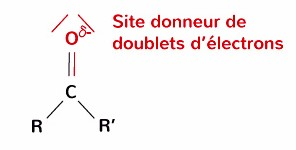
\includegraphics[width=.95\linewidth]{imgs/c4/donneur.jpg}  
\end{subfigure}
\begin{subfigure}{.45\textwidth}
  \centering
  %%%%%%%%%%%%%% include second image
  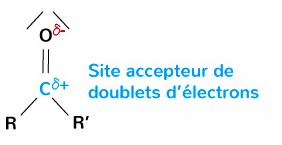
\includegraphics[width=.95\linewidth]{imgs/c4/accepteur.jpg}  
\end{subfigure}
\caption{Exemple de site donneur/accepteur dans une molécule. }
\end{figure}
Nous pouvons essayer de tout mettre ensemble maintenant et donner un modèle microscopique d'une réaction chimique par le billet de ce que l'on appelle un \textbf{mécanisme réactionnel}.

\begin{defn}{Mécanisme réactionnel}
\begin{itemize}
    \item Lors d’une transformation, l’\textbf{ensemble des réactions} qui se produisent au niveau microscopique constitue le mécanisme réactionnel.
    \item Chacune de ces réactions est \textbf{une étape du mécanisme réactionnel} et résulte de l’\textbf{interaction entre un site donneur et un site accepteur} de doublet d’électrons. 
    \item Le mouvement de ce doublet d’électrons peut être \textbf{représenté par une flèche courbe}, reliant le site donneur au site accepteur de doublet d’électrons. Ces flèches courbes permettent d’expliquer la formation ou la rupture des liaisons au cours de ces réactions. 
    \item Un mécanisme réactionnel peut se dérouler en \textbf{une seule étape, ou en plusieurs étapes}. Dans ce dernier cas, la formation et la rupture successive des liaisons font apparaître des entités chimiques temporaires appelées des \textbf{espèces intermédiaires}, avec une durée de vie moyenne de l’ordre de quelques picosecondes. 
\end{itemize}
\end{defn}

\begin{eg}
Une réaction avec une mécanisme en une seule étape
\begin{center}
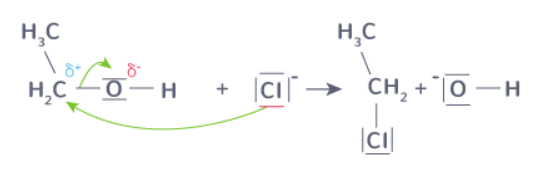
\includegraphics[width=0.7\linewidth]{imgs/c4/mecanisme1.png}    
\end{center}    
Un autre mécanisme avec une seule étape : 
\begin{center}
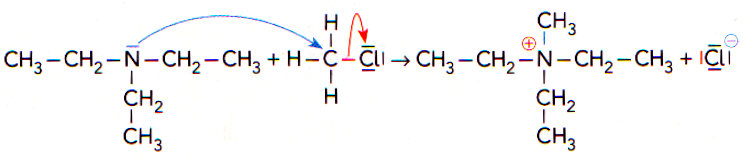
\includegraphics[width=0.7\linewidth]{imgs/c4/mecanisme3.jpg}    
\end{center} 
Un mécanisme multi-étapes: \begin{center}
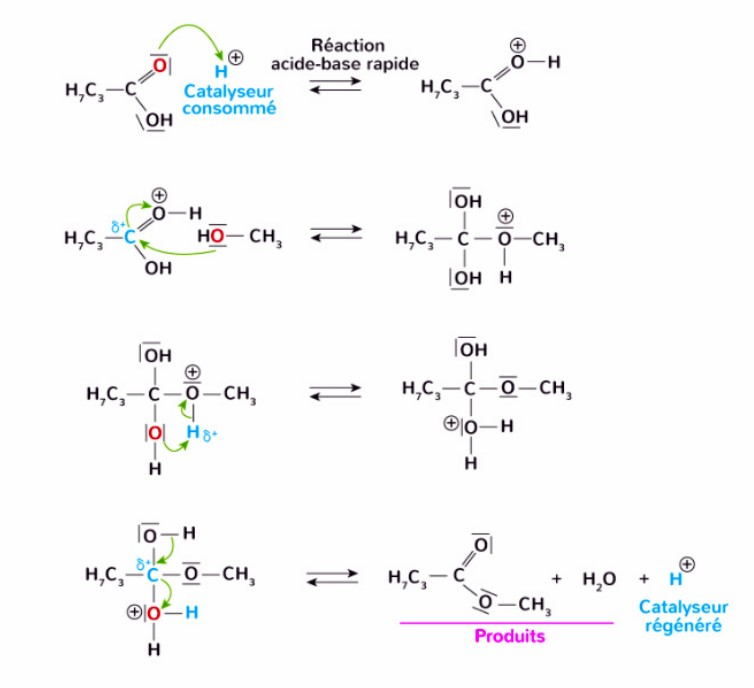
\includegraphics[width=0.7\linewidth]{imgs/c4/mecanisme2.jpg}    
\end{center} 
\end{eg}



\end{document}